\documentclass[convert = false, tikz]{standalone}
\usepackage[utf8]{inputenc}
\usepackage{tikz}
\usetikzlibrary{automata, positioning, arrows, shapes.geometric, decorations.pathmorphing}

\usepackage{../../../../style_automata}

% arara: pdflatex
% arara: latexmk: { clean: partial }
\begin{document}
    \tikzset{
    node distance=2cm, % specifies the minimum distance between two nodes.
    }
    \scalebox{0.8}{
    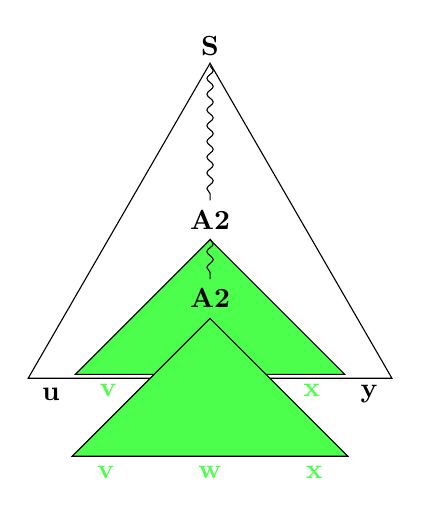
\begin{tikzpicture}

    % Apex angle 60 degrees
    \node[isosceles triangle, rotate=90, isosceles triangle apex angle=60, draw, minimum size=4cm] (T) {};
    \draw[] ([yshift=0.2cm]T.apex) node[](S){\textbf{S}};
    \draw[] ([yshift=-2cm]T.apex) node[](A2){\textbf{A2}};
    \draw[] (A2.south) node[isosceles triangle, rotate=90, isosceles triangle apex angle=90, draw, minimum size=1.71cm, anchor=apex, fill=green!70] (T2) {};
    \draw[] ([yshift=-1cm]A2) node[](A22){\textbf{A2}};
    \draw[] (A22.south) node[isosceles triangle, rotate=90, isosceles triangle apex angle=90, draw, minimum size=1.75cm, anchor=apex, fill=green!70] (T22) {};
    
    \draw[] ([yshift=-0.2cm,xshift=0.3cm]T.left corner) node[](u){\textbf{u}};
    \draw[] ([yshift=-0.2cm]T2.118) node[color=green!70](v){\textbf{v}};
    \draw[] ([yshift=-0.2cm]T22.118) node[color=green!70](v2){\textbf{v}};
    \draw[] ([yshift=-0.2cm]T22.lower side) node[color=green!70](w){\textbf{w}};
    \draw[] ([yshift=-0.2cm]T22.242) node[color=green!70](x2){\textbf{x}};
    \draw[] ([yshift=-0.2cm]T2.242) node[color=green!70](x){\textbf{x}};
    \draw[] ([yshift=-0.2cm,xshift=-0.3cm]T.right corner) node[](y){\textbf{y}};

    \draw [decorate,decoration={snake,amplitude=.4mm,segment length=2mm,post length=0mm}] (S.south) -- (A2.north);
    \draw [decorate,decoration={snake,amplitude=.4mm,segment length=2mm,post length=0mm}] (A2.south) -- (A22.north);
    
    \end{tikzpicture}
    }
\end{document}